\documentclass[dvipsnames,border=3pt]{standalone}
\usepackage{tikz}
\usetikzlibrary{arrows}
\usetikzlibrary{shapes}
\usepackage{enumitem}
\usepackage{bm}
\usepackage{mathdots}
\usepackage{amsmath}
\usetikzlibrary{shadings}
\usetikzlibrary{decorations.pathreplacing}
\usepackage{helvet}
\usetikzlibrary{arrows.meta}
\usepackage{graphicx}
\usepackage{pgfplots}
\usepackage{pgfplotstable}
\usepackage{filecontents}
\usetikzlibrary{plotmarks}
\usetikzlibrary{shapes.misc}
\pgfplotsset{compat=newest}

\renewcommand{\familydefault}{\sfdefault}

\definecolor{mylightgray}{cmyk}{0,0,0,0.1}
\usetikzlibrary{arrows,decorations.pathmorphing,backgrounds,fit,positioning,shapes.symbols,chains}

\begin{document}

\begin{tikzpicture}
    % trim=left botm right top
    
    %\node at (4.5,2.4) {\LARGE \textbf{GWAS data: interactions and main effects}};
    
    % 1 - 2
    \draw[-latex, line width=1mm,draw=gray!70] (3.62,0) -- (5.23,0);
    
    % 2 - 3
    \draw[-latex, line width=1mm,draw=gray!70] (9,-1.76) -- (9,-2.67);

    % 3 - 4
    \draw[-latex, line width=1mm,draw=gray!70] (-1.5,-7.93) -- (-1.5,-8.83);
    
    % 4 - 5
    \draw[-latex,line width=1mm,draw=gray!70] (-1.55,-11.33) -- (-1.55,-12.15);
    
    % 5 - 6
    \draw[-latex,line width=1mm,draw=gray!70] (1,-16.9) -- (1,-17.74);
    
    % 6 - 8
    \draw[-latex,line width=1mm,draw=gray!70] (4.2,-19.71) -- (5.77,-19.71);
    
    % 7 - 8
    \draw[-latex,line width=1mm,draw=gray!70] (8.08,-16.15) -- (8.08,-18.79);
    
    \node at (0,0) (1) {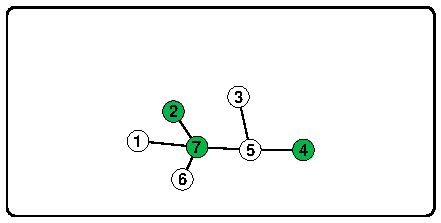
\includegraphics[clip,trim=0.1cm 0.1cm 0.1cm 0.1cm]{interaction_simulation1.pdf}};
    
    \node at (9,0) (2) {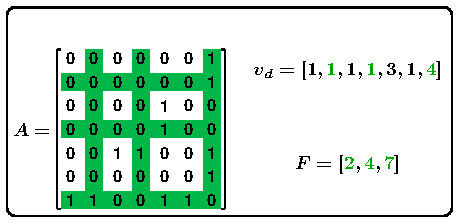
\includegraphics[clip,trim=0.1cm 0.1cm 0.1cm 0.1cm]{interaction_simulation2.pdf}};
    
    \node at (4.5,-5.3) (3) {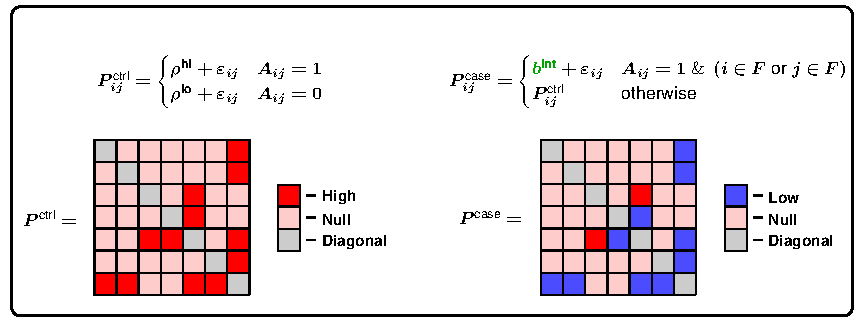
\includegraphics[clip,trim=0.1cm 0.1cm 0.1cm 0.1cm]{interaction_simulation3.pdf}};
    
    \node at (-1.5,-10.08) (4) {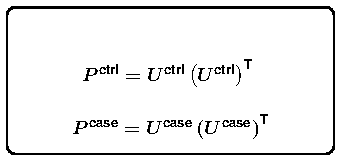
\includegraphics[clip,trim=0.1cm 0.1cm 0.1cm 0.1cm]{interaction_simulation4.pdf}};
    
    \node at (-1.55,-14.52) (5) {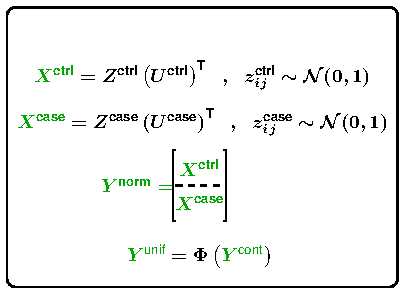
\includegraphics[clip,trim=0.1cm 0.1cm 0.1cm 0.1cm]{interaction_simulation5_gwas.pdf}};
    
    \node at (1,-19.71) (6) {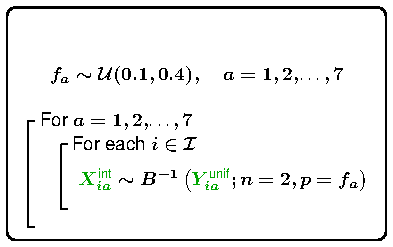
\includegraphics[clip,trim=0.1cm 0.1cm 0.1cm 0.1cm]{interaction_simulation6_gwas.pdf}};
    
    \node at (7.98,-13.02) (7) {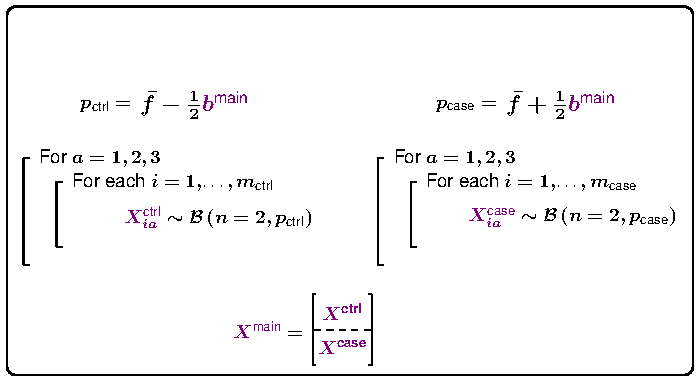
\includegraphics[clip,trim=0.1cm 0.1cm 0.1cm 0.1cm]{main_effect_gwas2.pdf}};
    
    \node at (8.08,-19.71) (8) {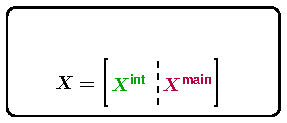
\includegraphics[clip,trim=0.1cm 0.1cm 0.1cm 0.1cm]{mixed_effects_combining_main-interaction.pdf}};
    
    %%%%%%%%%%%%%%%%%%%%%%%%%%%%%%%%%%%%%%% box 1 %%%%%%%%%%%%%%%%%%%%%%%%%%%%%%%%%%%%%%%%%%%%%%%
    \node[circle,draw,line width=0.2mm,xscale=1.4,yscale=1.4,fill=gray!40] at (-3.3,1.45) {};
    \node at (-3.3,1.45) {\textbf{1}};
    
    \node[xscale=1,yscale=1] at (0,0.9) {\textbf{Erd\H{o}s-R\'{e}nyi or Scale-free}};
    %\node[xscale=1,yscale=1] at (2.28,0.9) {\textbf{Erdos-Renyi}};
    %\node[xscale=1,yscale=1] at (0,0.9) {\textbf{or}};
    \node[xscale=1,yscale=1] at (0,1.45) {\textbf{Random graph}};
    %%%%%%%%%%%%%%%%%%%%%%%%%%%%%%%%%%%%%%% box 1 %%%%%%%%%%%%%%%%%%%%%%%%%%%%%%%%%%%%%%%%%%%%%%%
    
    %%%%%%%%%%%%%%%%%%%%%%%%%%%%%%%%%%%%%%% box 2 %%%%%%%%%%%%%%%%%%%%%%%%%%%%%%%%%%%%%%%%%%%%%%%
    \node[circle,draw,line width=0.2mm,xscale=1.4,yscale=1.4,fill=gray!40] at (5.55,1.45) {};
    \node at (5.55,1.45) {\textbf{2}};
    
    \node[xscale=1,yscale=1] at (7.5,1.45) {\textbf{Adjacency matrix}};
    \node[xscale=1,yscale=1] at (11,1.2) {\textbf{Degree vector}};
    \node[xscale=1,yscale=1] at (11,-0.4) {\textbf{Interaction features}};
    %%%%%%%%%%%%%%%%%%%%%%%%%%%%%%%%%%%%%%% box 2 %%%%%%%%%%%%%%%%%%%%%%%%%%%%%%%%%%%%%%%%%%%%%%%
    
    %%%%%%%%%%%%%%%%%%%%%%%%%%%%%%%%%%%%%%% box 3 %%%%%%%%%%%%%%%%%%%%%%%%%%%%%%%%%%%%%%%%%%%%%%%
    \node[circle,draw,line width=0.2mm,xscale=1.4,yscale=1.4,fill=gray!40] at (-2.3,-3.01) {};
    \node at (-2.3,-3.01) {\textbf{3}};
    
    \node[xscale=1,yscale=1] at (4.5,-2.94) {\textbf{Correlation matrices}};
    
    \node[xscale=1,yscale=1] at (0.1,-4.7) {\textbf{Controls}};
    \node[xscale=1,yscale=1] at (7.6,-4.7) {\textbf{Cases}};
    %%%%%%%%%%%%%%%%%%%%%%%%%%%%%%%%%%%%%%% box 3 %%%%%%%%%%%%%%%%%%%%%%%%%%%%%%%%%%%%%%%%%%%%%%%
    
    %%%%%%%%%%%%%%%%%%%%%%%%%%%%%%%%%%%%%%% box 4 %%%%%%%%%%%%%%%%%%%%%%%%%%%%%%%%%%%%%%%%%%%%%%%
    \node[circle,draw,line width=0.2mm,xscale=1.4,yscale=1.4,fill=gray!40] at (-3.96,-9.16) {};
    \node at (-3.96,-9.16) {\textbf{4}};
    \node[xscale=1,yscale=1] at (-1.3,-9.13) {\textbf{Cholesky decomposition}};
    %%%%%%%%%%%%%%%%%%%%%%%%%%%%%%%%%%%%%%% box 4 %%%%%%%%%%%%%%%%%%%%%%%%%%%%%%%%%%%%%%%%%%%%%%%
    
    %%%%%%%%%%%%%%%%%%%%%%%%%%%%%%%%%%%%%%% box 5 %%%%%%%%%%%%%%%%%%%%%%%%%%%%%%%%%%%%%%%%%%%%%%%
    \node[circle,draw,line width=0.2mm,xscale=1.4,yscale=1.4,fill=gray!40] at (-4.535,-12.47) {};
    \node at (-4.535,-12.47) {\textbf{5}};
    \node[xscale=1,yscale=1] at (-1.55,-12.42) {\textbf{Correlated continuous data}};
    %%%%%%%%%%%%%%%%%%%%%%%%%%%%%%%%%%%%%%% box 5 %%%%%%%%%%%%%%%%%%%%%%%%%%%%%%%%%%%%%%%%%%%%%%%
    
    %%%%%%%%%%%%%%%%%%%%%%%%%%%%%%%%%%%%%%% box 6 %%%%%%%%%%%%%%%%%%%%%%%%%%%%%%%%%%%%%%%%%%%%%%%
    \node[circle,draw,line width=0.2mm,xscale=1.4,yscale=1.4,fill=gray!40] at (-1.903,-18.05) {};
    \node at (-1.903,-18.05) {\textbf{6}};
    \node[xscale=1,yscale=1] at (1,-18.01) {\textbf{Interaction data}};
    %%%%%%%%%%%%%%%%%%%%%%%%%%%%%%%%%%%%%%% box 6 %%%%%%%%%%%%%%%%%%%%%%%%%%%%%%%%%%%%%%%%%%%%%%%
    
    %%%%%%%%%%%%%%%%%%%%%%%%%%%%%%%%%%%%%%% box 7 %%%%%%%%%%%%%%%%%%%%%%%%%%%%%%%%%%%%%%%%%%%%%%%
    \node[circle,draw,line width=0.2mm,xscale=1.4,yscale=1.4,fill=gray!40] at (2.48,-10.22) {};
    \node at (2.48,-10.22) {\textbf{7}};
    \node[xscale=1,yscale=1] at (7.98,-10.18) {\textbf{Main effect data}};
    
    \node[xscale=1,yscale=1] at (4.75,-10.93) {\textbf{Controls}};
    
    \node[xscale=1,yscale=1] at (10.75,-10.93) {\textbf{Cases}};
    %%%%%%%%%%%%%%%%%%%%%%%%%%%%%%%%%%%%%%% box 7 %%%%%%%%%%%%%%%%%%%%%%%%%%%%%%%%%%%%%%%%%%%%%%%
    
    %%%%%%%%%%%%%%%%%%%%%%%%%%%%%%%%%%%%%%% box 8 %%%%%%%%%%%%%%%%%%%%%%%%%%%%%%%%%%%%%%%%%%%%%%%
    \node[circle,draw,line width=0.2mm,xscale=1.4,yscale=1.4,fill=gray!40] at (6.07,-19.09) {};
    \node at (6.07,-19.09) {\textbf{8}};
    \node[xscale=1,yscale=1] at (8.08,-19.05) {\textbf{Mixed effects data}};
    %%%%%%%%%%%%%%%%%%%%%%%%%%%%%%%%%%%%%%% box 8 %%%%%%%%%%%%%%%%%%%%%%%%%%%%%%%%%%%%%%%%%%%%%%%
    
\end{tikzpicture}
    
\end{document}